%datadasedesign.tex
The database is designed in MySQL 5.1.61, and resembles the local database created by the ``Admin-group'' very closely -- the only difference is, that the Savanah database has two extra fields in the ``AuthUsers'' table: username and password. The reason for this is, that while all apps running on the android platform uses QR-codes for user authentication, this is not a fitting choice for the webinterface; it would be more complicated to scan the QR-code form a webcam to login, than to simply use a username and password combination.

\subsubsection{Requirements}
The requirements for the database has been provided by the app groups, and are as follows:

\begin{itemize}
	\item All users must be able to login with a QR-code
	\item Each department must also be able to login
	\item All users must be linked to at least one department
	\item All guardians must be able to be linked to at least one child.
	\item All parents must be able to be linked to at least one child.
	\item All users must be able to have access all the apps
	\item All users must be able to access their own pictures, and all public pictures
	\item All departments must be able to access all public pictures
	\item All pictures needs to be able to be linked to different tags
	\item Pictures must be able to be linked with audio and vice versa
	\item A department must be able to have a subdepartment\footnote{Example: ``Birken'' has two departments, at two different addresses, both these subdepartments needs to be linked with ``Birken'' as a superdepartment}
\end{itemize}

\subsubsection*{Diagram}
A diagram has been made to get a overview of the different tables and their relations. This diagram is designed in DIA, which is a GTK+ based diagram creation program\cite{Dia}, and can be seen in \autoref{fig:DiaDesign}.

\begin{figure}[htbp]
	\centering
		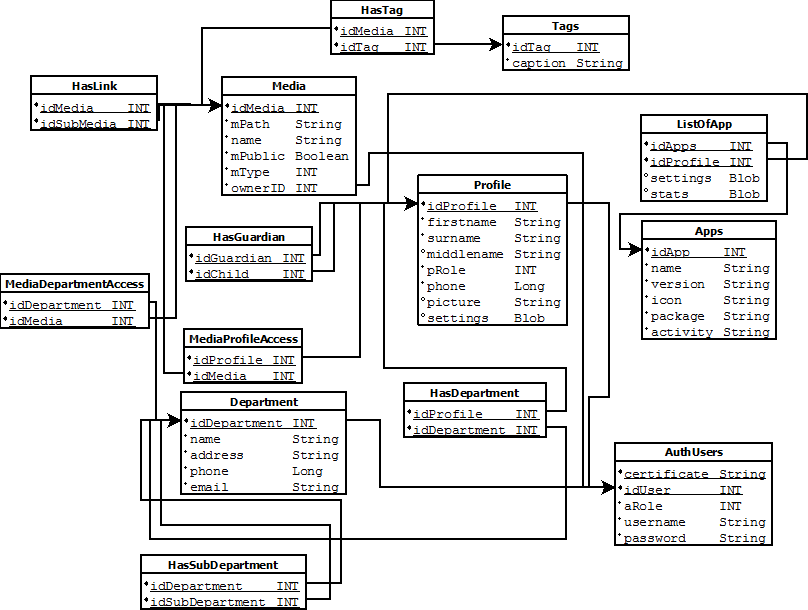
\includegraphics[width=1.00\textwidth]{images/DiaDesign.png}
	\caption{Dia diagram of the database}
	\label{fig:DiaDesign}
\end{figure}

Although the diagram in \autoref{fig:DiaDesign} does not meet the standard of database diagrams, it does provide a good view of the different tables, and the relations: Foreign keys points to where the value is fetched form. This crude diagram shows that be having the ``idUser'' from the ``AuthUsers'' one is able to access all other information for that specific user.

\subsubsection{Normal form}
To prevent modification anomalies in the database, it can be normalized. This becomes important when a table is dealing with functional dependencies. The solution is to remove the dependicies form the table to another (e.g. split a table into two). An example of this is shown in \autoref{tab:nonNormalizedExample} and \autoref{tab:NormalizedDatabaseExample}.

\begin{table}[htbp]
	\centering
		\begin{tabular}{|c|c|c|}
		\hline
		 \multicolumn{3}{|c|}{Sales}\\
		\multicolumn{1}{|c}{Customer\_ID} & \multicolumn{1}{c}{Product} & \multicolumn{1}{c|}{Price} \\
		\hline
		1001 & Laundry detergent & 12 \\ \hline
		1007 & Toothpaste & 3 \\ \hline
		1010 & Chlorine bleach & 4 \\ \hline
		1024 & Toothpaste & 3\\	\hline
		\end{tabular}
	\caption{Non-normalized database\cite[p. 114]{sqlForDummies}}
	\label{tab:nonNormalizedExample}
\end{table}

The problem in \autoref{tab:nonNormalizedExample} is, that if customer 1001 is removed form the database, not only his products are removed, but the fact that Laundry detergent costs 12\$ is also lost. A way to cope with this, is to split the table into two tables, as seen in \autoref{tab:NormalizedDatabaseExample}

\begin{table}[htbp]
	\centering
		\begin{tabular}{c c}
			\begin{tabular}{|c|c|}
				\hline
		 		\multicolumn{2}{|c|}{CUST\_PURCH} \\
		 		\multicolumn{1}{|c}{Customer\_ID} & \multicolumn{1}{c|}{Product} \\
		 		\hline
		 		1001 & Laundry detergent \\ \hline
		 		1007 & Toothpaste \\ \hline
		 		1010 & Chlorine bleach \\ \hline
		 		1024 & Toothpaste \\ \hline
			\end{tabular}
		&
			\begin{tabular}{|c|c|}
				\hline
				\multicolumn{2}{|c|}{PROD\_PRICE} \\
				\multicolumn{1}{|c}{Product} & \multicolumn{1}{c|}{Price} \\
				\hline
				Laundry detergent & 12 \\ \hline
				Toothpaste & 3 \\ \hline
				Chlorine bleach & 4 \\ \hline
			\end{tabular}
		\end{tabular}
	\caption{Normalized database example\cite[p 115]{sqlForDummies}}
	\label{tab:NormalizedDatabaseExample}
	\end{table}

As seen in \autoref{tab:NormalizedDatabaseExample} the table ``CUST\_PURCH'' now only deals with the customer, and thus it is no possible to remove a customer form the system, without loosing the data about the product.

There are several degrees of normal form for a database, here the focus is on the first three (1st, 2nd and 3rd normal form).

\subsubsection{First normal form (1NF)}
The example in \autoref{tab:nonNormalizedExample} and \autoref{tab:NormalizedDatabaseExample}, is an example of 1NF. To achieve this the following rules must apply\cite[p. 116]{sqlForDummies}:
\begin{itemize}
	\item Each cell (intersection of a row and a column) of the table must have only a single value.
	\item Each column must have a unique name.
	\item No two rows may be identical (that is, each row must be unique).
	\item Each column contains data for a single attribute of the thing it's describing.
\end{itemize}

As seen in \autoref{fig:DiaDesign} the Savannah database is follows the rules for 1NF, and thus is 1NF.

\subsubsection{Second normal form (2NF)}
For the database to be in 2NF, if a table does contain a composite key, all other attributes in the table must be depended on the entire key.
Furthermore \cite[p. 117]{sqlForDummies} states:
\begin{quotation}
...every
relation that is in 1NF with a single attribute key is automatically in second
normal form.
\end{quotation}
As this is the case in the Savannah database it is in 2NF.

\subsubsection{Third normal form (3NF)}
For a database to be en 3NF, it is required that there are no transitive dependency\footnote{A transitive dependency occurs when one attribute depends on a second
attribute, which depends on a third attribute. Deletions in a table with such a
dependency can cause unwanted information loss. \cite[p. 118]{sqlForDummies}}.
As seen in \autoref{fig:DiaDesign} does live up to this definition. There are no transitive dependencies within any of the tables. A good example of this is the handling of a ``Profile'''s access to ``Apps'': When the app is removed from the ``Profile'' it is done in the ``ListOfApps'' table, and thus only the relation is removed, and the specific app still is available in the system. This makes the Savannah database to be in 3NF.



\subsubsection*{Rules}
\label{databaseRules}
To provide the security needed in the system, a few rules need to apply for the databse:
\begin{itemize}
	\item The ``Profile''$\rightarrow$''AuthUsers'' relation must be one-to-one, as one user form the ``AuthUsers'' can only have one profile in the system
	\item The ``Department''$\rightarrow$''AuthUsers'' relation must be one-to-one, as one department form the ``AuthUsers'' can only be one department in the system
	\item The ``idUser'' in ``AuthUsers'' must be unique.
	\item The ``username'' in ``AuthUsers'' must be unique
	\item It must be possible to distinguish between users and departments in the ``AuthUsers'' table
	\item It must be possible to distinguish between children, parents and guardians in the ``Profile'' table
\end{itemize}

These rules will be applied in a mix between SQL script and software level in \textbf{REF TIL SECTION}